%Korrekturgelesen : Sophie Dietrich
\chapter{Recherche}

\section{Ethersex}

Auf der Projekt-Website (\url{http://ethersex.de}) bewirbt sich Ethersex als
\begin{quote} \textit{
		\enquote{[\ldots] eine Firmware mit Netzwerkunterstützung für 8-bit AVR
		Mikrocontroller, die durch eine Community entwickelt wird.  }
	}
	\cite{Ethersex}
\end{quote}

Ethersex unterstützt sowohl die von uns verwendeten ATmega Prozessoren, das
AVR-Net-IO Board und auch den verwendeten ENC28J60 Netzwerk Controller.
Durch einen ausführlichen Quick Start Guide
(\url{http://ethersex.de/index.php/Quick_Start_Guide/Preparation}) auf der
Projektseite ist es, auch für Anfänger in diesem Themengebiet, sehr einfach möglich, das Projekt lauffähig zu machen. 
Fast die gesamte Konfiguration kann über ein Menü vorgenommen werden. So muss nicht wie beim Radig Projekt zum
ändern der Mac Adresse in eine Headerdatei geschrieben werden. 

\begin{figure}[H]
	\centering
		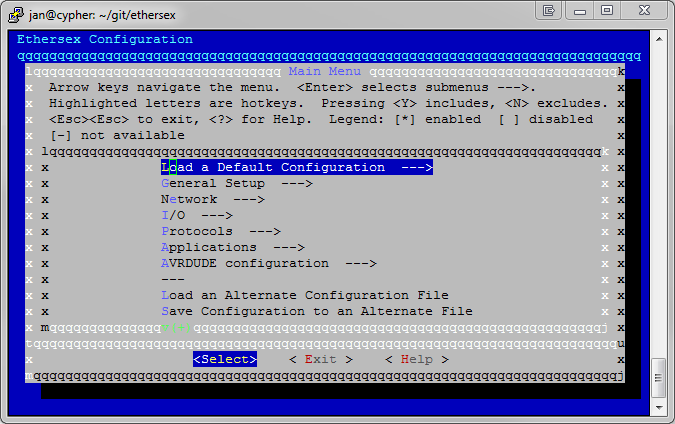
\includegraphics[width=13cm]{content/pictures/Recherche/Ethersex/Ehtersex1.png}
	\caption{Ethersex menuconfig}
	\label{Ethersex1}
\end{figure} 

Im Bild (Abb. \ref{Ethersex1}) sieht man den Startbildschirm des
Menüs, das über den Befehl \textrm{make menuconfig} erreicht werden kann.
Hier können verschiedene Einstellungen getroffen werden. Zum Beispiel, den
verwendeten Mikrocontroller, welche Mac Adresse der Netzwerk Controller
verwendet oder welche IP Adresse gewünscht ist.
Nachdem die Konfiguration abgeschlossen ist, kann das Hexfile mit dem
\textrm{make} Befehl erstellt werden. In der Abbildung \ref{Ethersex2} sieht man,
dass am Ende des \textrm{Make} Prozesses die aktuelle Größe des erstellten Binary Datei
angezeigt wird.

\begin{figure}[H]
	\centering
		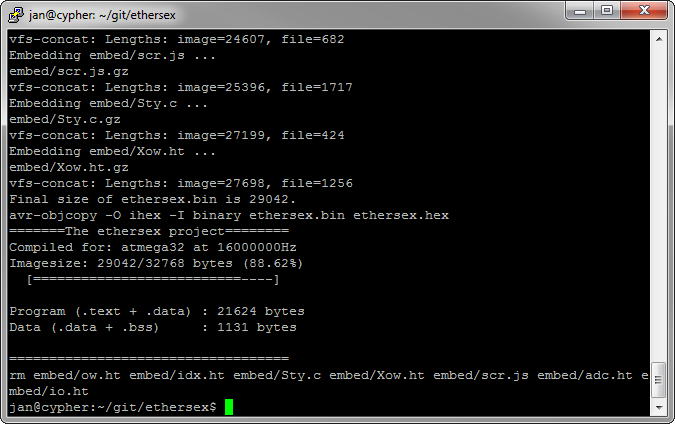
\includegraphics[width=13cm]{content/pictures/Recherche/Ethersex/Ethersex2.png}
	\caption{Ethersex make project}
	\label{Ethersex2}
\end{figure} 

Das Einbinden der Website beim Ethersex Projekt wird in der Anleitung
folgendermaßen beschrieben:

\begin{quote}
	\textit{
		\enquote{Falls die Option Supply Inline Files aktiviert ist, werden alle
		Dateien, die unter vfs/embed/ abgelegt sind, automatisch beim Erstellen des
		Images mit gzip gepackt und an das Ende der Firmware angehängt. Die
		Dateinamen bleiben dabei unverändert [\ldots]} }
	\cite[\url{http://www.ethersex.de/index.php/HTTPD_(Deutsch)}]{Ethersex}
\end{quote}

\section{Elektronik 2000}

Einen anderen Ansatz verfolgt das Projekt Elektronik 2000.
Hier wird nicht nur der Webserver geboten sondern eine erweiterte GUI, um das
Board zu programmieren. Dafür wird mit einem grafischem Designer eine Logik
entworfen und über einen ISP Programmer auf das Board gebracht.

\begin{quote}
	\textit{
		\enquote{Das E2000-NET-IO basiert auf dem AVR-NET-IO von Pollin. Durch die
		E2000-Firmware wird aus dem AVR-NET-IO von Pollin ein autak laufendes
		Logikmodul. Mit diesem Modul können über Netzwerk Schaltvorgänge ausgeführt
		werden. Außerdem sind Zeitgesteuerte Schaltvorgänge möglich.} }
	\cite{elektronik2000}
\end{quote}

Durch die Netzwerkanbindung des AVR-Net-IO kann dann die programmierte Logik von
außen überwacht und gesteuert werden. Dafür gibt es von den Entwicklern eine
bereitgestellte Android Applikation. Zusätzlich zu einem Projekt das mit dem
AVR-Net-IO arbeitet gibt es mittlerweile eine weitere Version, welche auch mit dem
Raspberry Pi zusammenarbeitet und die GPIO Pins des Pis nach außen steuerbar
macht.

\section{Ulrich Radig}

Ein weiteres Projekt für den AVR-Net-IO ist die AVR Webserver Software
(\url{http://www.ulrichradig.de/home/index.php/software/avr-webserver-software}).
Die Software ist ein Webserver für die Mikrocontroller der Baureihen ATmega 32,
64 und 128. Durch die Einfache Bindung der Dateien kann das Projekt
einfach an eigene Bedürfnisse angepasst werden. Dabei hat die Software noch
weiter Funktionalität:

\begin{itemize}
  \item \textbf{\ac{HTTP} Server} Webserver ohne Dateistruktur
  \item \textbf{Sendmail} Senden von E-Mails
  \item \textbf{Weather} Ermitteln von Wetterdaten
  \item \textbf{\ac{NTP}} Empfangen von Internetzeit
  \item \textbf{\ac{DNS}} Beantwortung von Anfragen zur
  Namensauflösung
  \item \textbf{\ac{USART}} eine Schnittstelle im Mikrocontroller zum
  Datenaustausch mit PC über die COM-Schnittstelle
  \item \textbf{\ac{Telnet}} zeichenorientierter
  Datenaustausch über eine TCP-Verbindung.
  \item \textbf{\ac{CMD}} Verwaltung der Telnet-Konsolenbefehle.
  \item \textbf{\ac{WOL}} Funktionalität um andere Geräte im Netzwerk
  durch bestimmte Datenpakete aufzuwecken.
\end{itemize}
